

\documentclass[letterpaper, 10 pt, conference]{ieeeconf}  

\IEEEoverridecommandlockouts
%\overrideIEEEmargins
%See the \addtolength command later in the file to balance the column lengths on the last page of the document

% The following packages can be found on http:\\www.ctan.org
%\usepackage{graphics} % for pdf, bitmapped graphics files
%\usepackage{epsfig} % for postscript graphics files
%\usepackage{mathptmx} % assumes new font selection scheme installed
%\usepackage{times} % assumes new font selection scheme installed
%\usepackage{amsmath} % assumes amsmath package installed
%\usepackage{amssymb}  % assumes amsmath package installed
\usepackage{graphicx}

\title{\huge \bf
CoSTAR in Surgery: A Cross-platform User Interface \\for Collaborative Robot Task Specification
}
%
\author{Baichuan Jiang$^{1}$ and Chris Paxton$^{2}$
\thanks{$^{1}$H. Kwakernaak is with Faculty of Electrical Engineering, Mathematics and Computer Science,
        University of Twente, 7500 AE Enschede, The Netherlands
        {\tt\small h.kwakernaak at papercept.net}}
\thanks{$^{2}$P. Misra is with the Department of Electrical Engineering, Wright State University,
        Dayton, OH 45435, USA
        {\tt\small p.misra at ieee.org}}%
}

\begin{document}

\maketitle
\thispagestyle{empty}
\pagestyle{empty}


%%%%%%%%%%%%%%%%%%%%%%%%%%%%%%%%%%%%%%%%%%%%%%%%%%%%%%%%%%%%%%%%%%%%%%%%%%%%%%%%
\begin{abstract}

Human-Robot Collaboration (HRC) in surgery have been an emerging field of study in recent years, which aims at incorporating both surgeon and machine’s advantages to improve safety, accuracy and speed. In this work, we propose a cross-platform, open-source framework that would facilitate the surgical HRC research. The work is based on CoSTAR, which originally aims at allowing small manufacturers to easily specify complex tasks for robots accommodating different task scenarios. To demonstrate its feasibility as a platform for collaborative surgical robot research, we generalized the original system and implemented it on da Vinci Research Kit (dVRK), while maintains its full functionality on other robot platforms such as UR5 and KUKA LBR iiwa.  

\end{abstract}


%%%%%%%%%%%%%%%%%%%%%%%%%%%%%%%%%%%%%%%%%%%%%%%%%%%%%%%%%%%%%%%%%%%%%%%%%%%%%%%%
\section{Introduction}

Surgical robots have been increasingly adopted in clinical procedures to support surgeons with various tasks, while most systems currently available are under full control of the surgeon. It is suggested in recent studies \cite{padoy2011human,berthet2016hubot,bauzano2016collaborative,hu2015semi} that incorporating further intelligence into the surgical robot will free surgeons from repetitive tasks, reduce large movements of master manipulator to avoid clutching and readjusting hand position, and achieve better overall precision and accuracy. 

For many of the proposed collaborative schemes, the central idea is to take advantage of the reliability in robots to perform less critical tasks while also allowing surgeons in the loop to perform fine actions with their domain knowledge. Hubot system in \cite{berthet2016hubot} runs continuously in a loop, alternating between three modes: fully manual, manual with haptic guidance, fully automated. Padoy et al. \cite{padoy2011human} adopted Hidden Markov Model (HMM) as a way of modeling surgical procedure. To automatically alternate between manual and automated subtasks, observations of surgeon’s movement is served as a trigger for next automated subtask. Collaboration system for HALS procedure \cite{bauzano2016collaborative} where surgeon inserts a hand into abdomen while operating the laparoscopic instrument using the other hand also utilizes a workflow manager to allow the robot being informed of the current state of intervention. Therefore, we propose a common task specification framework where tasks can be represented by nodes of behavior tree, corresponding to different phases in these collaborative schemes. 

This work is a surgical generalization of our previous work in \cite{paxton2017costar}, where the aim is to provide an easy way of authoring task plans for industrial robots such as UR5 and KUKA LBR iiwa. Therefore, while UR5 and KUKA LBR iiwa are also major platforms for collaborative surgical robot research, the focus of this work is on the new implementation on dVRK with syste setup shown in Fig.1. 


\begin{figure}[bt]
\centering
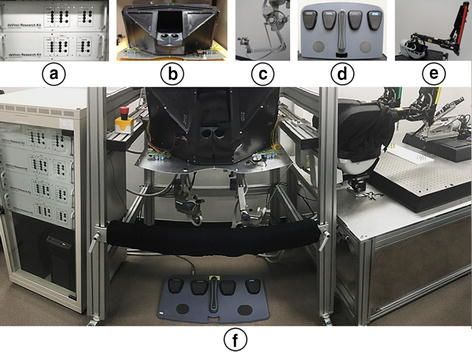
\includegraphics[width=150pt]{dvrk.jpg}
\caption{dVRK system setup (a placeholder).}
\label{fig:dvrk}
\end{figure}


\section{Methodology}



\section{Conclusions}

\addtolength{\textheight}{-12cm}   % This command serves to balance the column lengths
                                  % on the last page of the document manually. It shortens
                                  % the textheight of the last page by a suitable amount.
                                  % This command does not take effect until the next page
                                  % so it should come on the page before the last. Make
                                  % sure that you do not shorten the textheight too much.

%%%%%%%%%%%%%%%%%%%%%%%%%%%%%%%%%%%%%%%%%%%%%%%%%%%%%%%%%%%%%%%%%%%%%%%%%%%%%%%%



%%%%%%%%%%%%%%%%%%%%%%%%%%%%%%%%%%%%%%%%%%%%%%%%%%%%%%%%%%%%%%%%%%%%%%%%%%%%%%%%



%%%%%%%%%%%%%%%%%%%%%%%%%%%%%%%%%%%%%%%%%%%%%%%%%%%%%%%%%%%%%%%%%%%%%%%%%%%%%%%%
\section*{APPENDIX}

\section*{ACKNOWLEDGMENT}


%%%%%%%%%%%%%%%%%%%%%%%%%%%%%%%%%%%%%%%%%%%%%%%%%%%%%%%%%%%%%%%%%%%%%%%%%%%%%%%%

%References are important to the reader; therefore, each citation must be complete and correct. If at all possible, references should be commonly available publications.

\bibliographystyle{IEEEtran}
\bibliography{surgical}

\end{document}
